% begin module sequence-plotting
\begin{frame}
\begin{columns}[c]
\column{.5\textwidth}
\ \only<handout:0| -2>{%
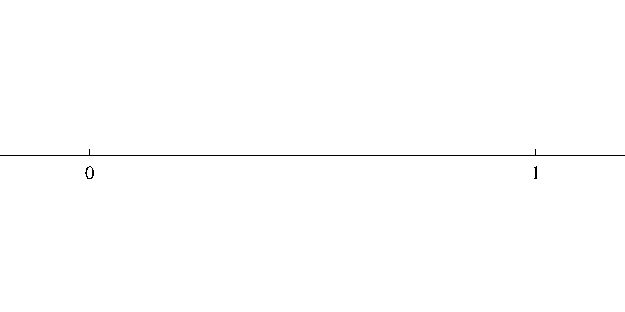
\includegraphics[width=5cm]{sequences/pictures/12-01-numberlinea.pdf}%
}%
\only<handout:0| 3>{%
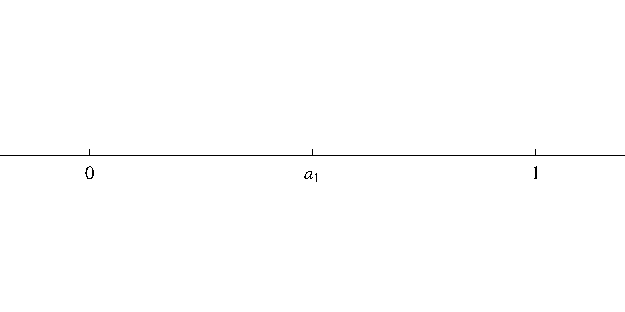
\includegraphics[width=5cm]{sequences/pictures/12-01-numberlineb.pdf}%
}%
\only<handout:0| 4>{%
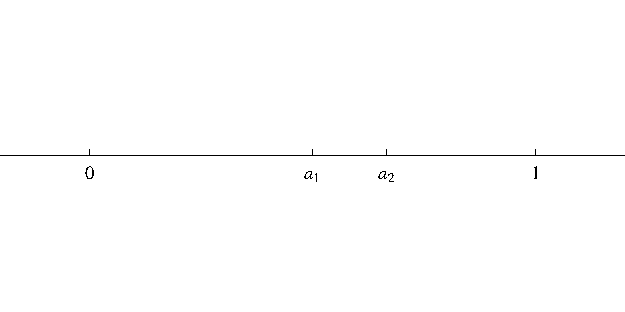
\includegraphics[width=5cm]{sequences/pictures/12-01-numberlinec.pdf}%
}%
\only<handout:0| 5>{%
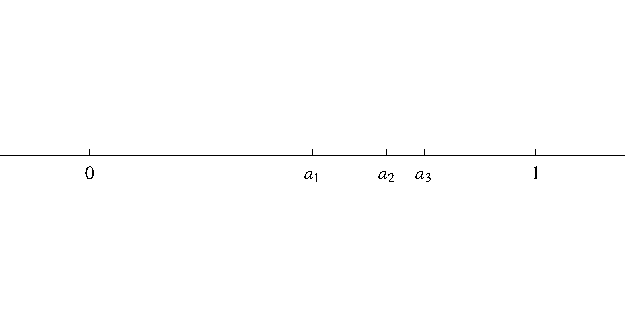
\includegraphics[width=5cm]{sequences/pictures/12-01-numberlined.pdf}%
}%
\only<handout:0| 6>{%
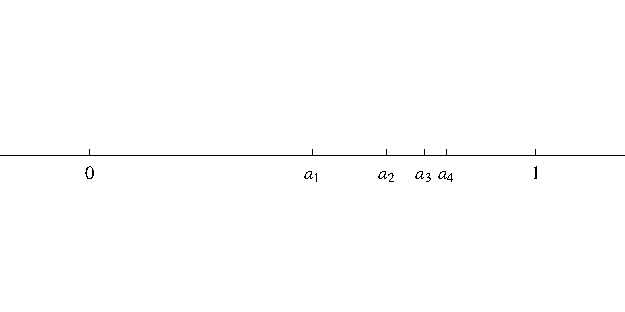
\includegraphics[width=5cm]{sequences/pictures/12-01-numberlinee.pdf}%
}%
\only<handout:0| 7>{%
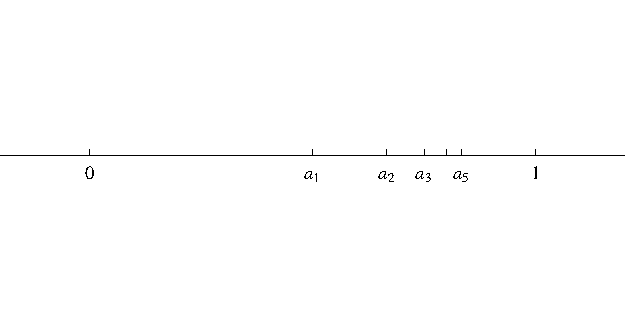
\includegraphics[width=5cm]{sequences/pictures/12-01-numberlinef.pdf}%
}%
\only<handout:0| 8>{%
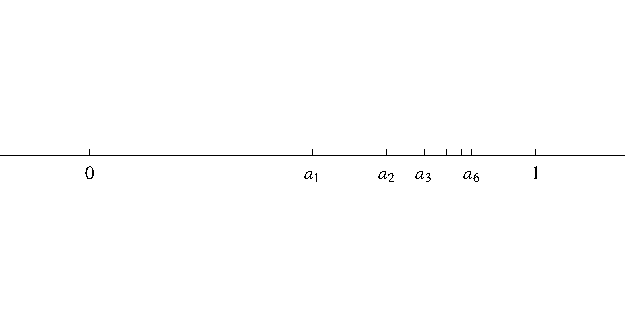
\includegraphics[width=5cm]{sequences/pictures/12-01-numberlineg.pdf}%
}%
\only<handout:0| 9>{%
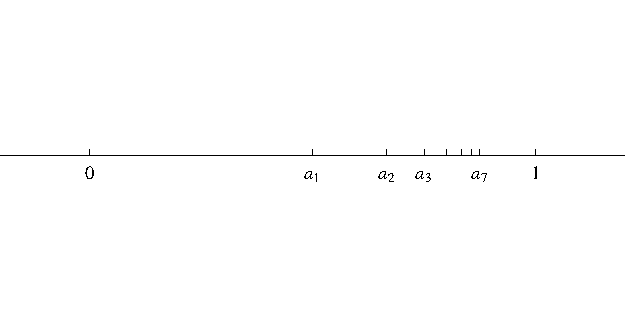
\includegraphics[width=5cm]{sequences/pictures/12-01-numberlineh.pdf}%
}%
\only<handout:0| 10>{%
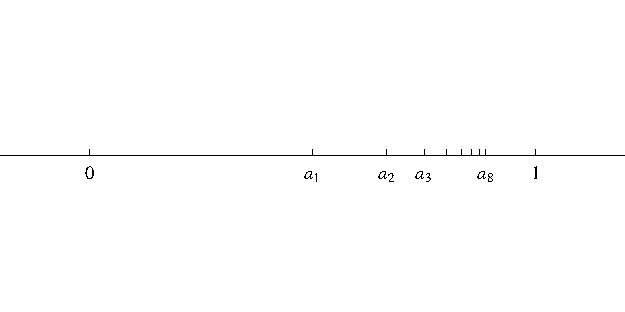
\includegraphics[width=5cm]{sequences/pictures/12-01-numberlinei.pdf}%
}%
\only<11->{%
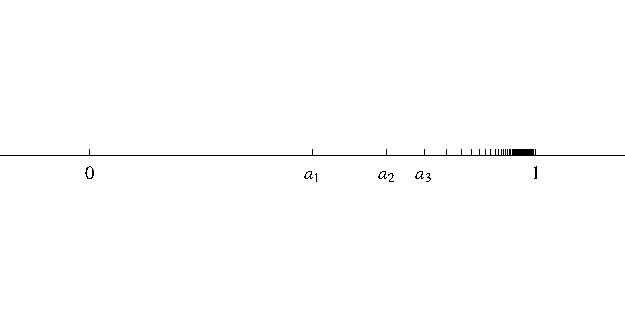
\includegraphics[width=5cm]{sequences/pictures/12-01-numberlinej.pdf}%
}%

Number line
\column{.5\textwidth}
\ \only<handout:0| -2>{%
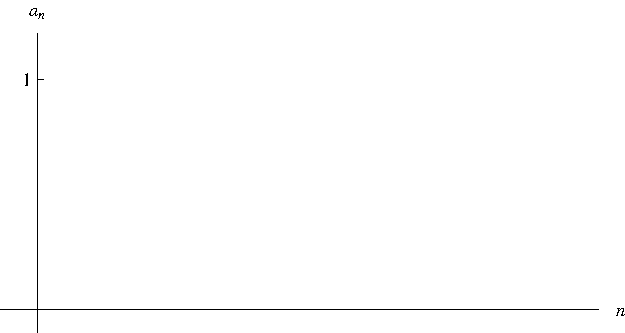
\includegraphics[width=6cm]{sequences/pictures/12-01-sequencegrapha.pdf}%
}%
\only<handout:0| 3>{%
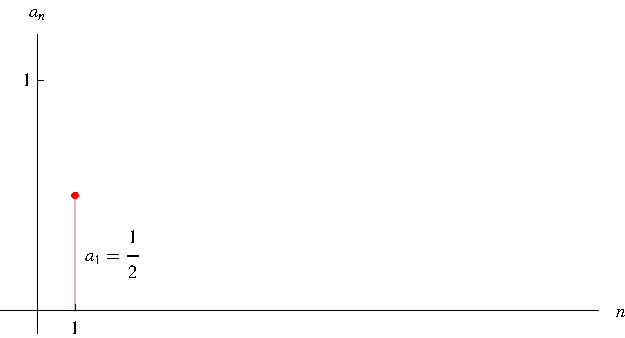
\includegraphics[width=6cm]{sequences/pictures/12-01-sequencegraphb.pdf}%
}%
\only<handout:0| 4>{%
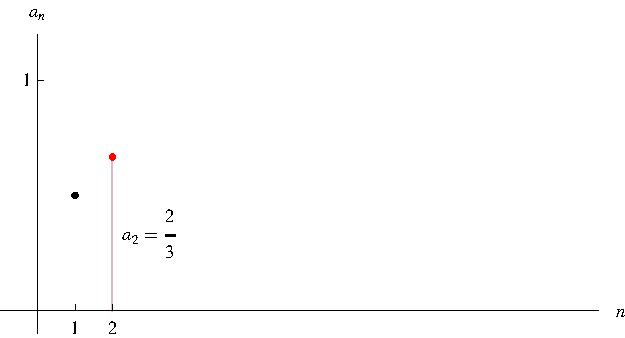
\includegraphics[width=6cm]{sequences/pictures/12-01-sequencegraphc.pdf}%
}%
\only<handout:0| 5>{%
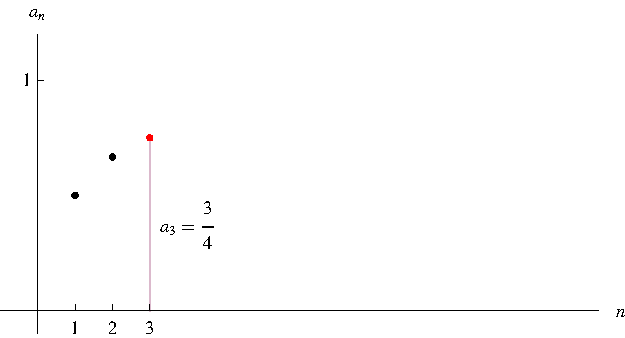
\includegraphics[width=6cm]{sequences/pictures/12-01-sequencegraphd.pdf}%
}%
\only<handout:0| 6>{%
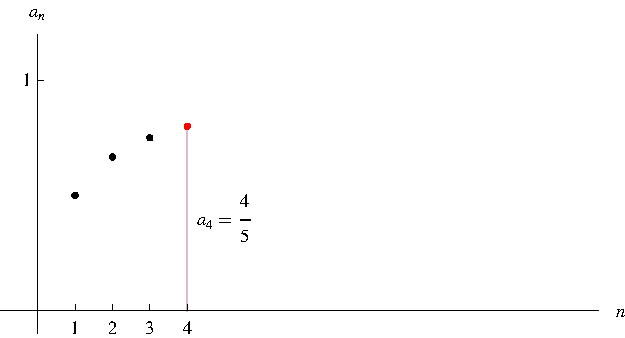
\includegraphics[width=6cm]{sequences/pictures/12-01-sequencegraphe.pdf}%
}%
\only<handout:0| 7>{%
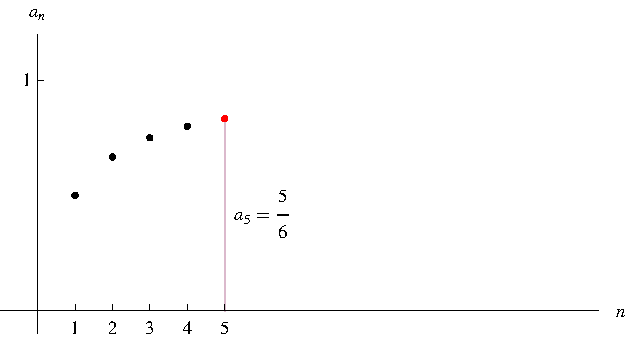
\includegraphics[width=6cm]{sequences/pictures/12-01-sequencegraphf.pdf}%
}%
\only<handout:0| 8>{%
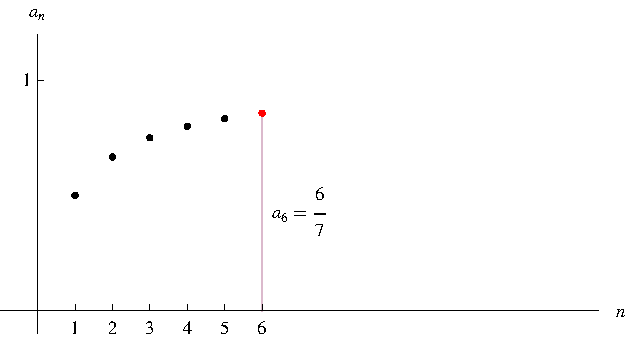
\includegraphics[width=6cm]{sequences/pictures/12-01-sequencegraphg.pdf}%
}%
\only<handout:0| 9>{%
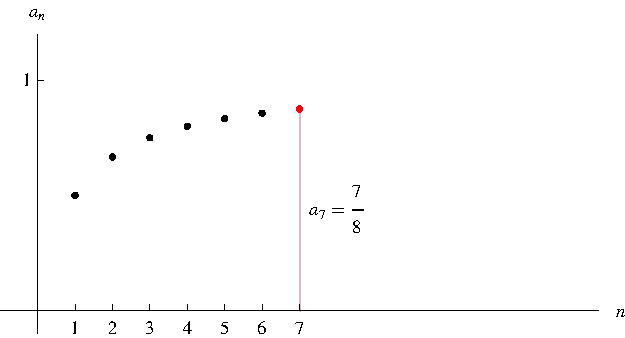
\includegraphics[width=6cm]{sequences/pictures/12-01-sequencegraphh.pdf}%
}%
\only<handout:0| 10>{%
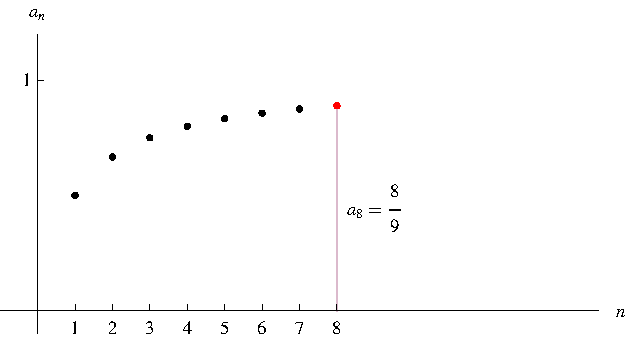
\includegraphics[width=6cm]{sequences/pictures/12-01-sequencegraphi.pdf}%
}%
\only<11->{%
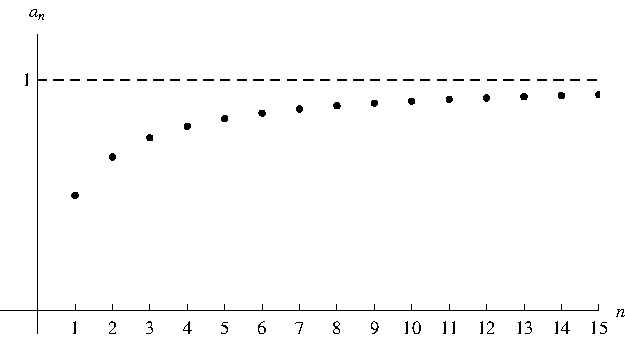
\includegraphics[width=6cm]{sequences/pictures/12-01-sequencegraphj.pdf}%
}%

Cartesian coordinates
\end{columns}
\begin{itemize}
\item  The sequence $\left\{ \frac{n}{n+1}\right\}$ can be plotted on a number line or using Cartesian coordinates.
\item<12->  From the pictures, the terms in the sequence appear to approach $1$ as $n$ gets larger.
\item<13->  \alert<handout:0| 13-14>{$1 - \frac{n}{n+1} =$ \uncover<14->{$\frac{1}{n+1}$.}}
\item<15->  This can be made arbitrarily small by choosing $n$ large enough.
\item<16->  We express this by writing $\lim_{n\to\infty}\frac{n}{n+1} = 1$.
\end{itemize}
\end{frame}
% end module sequence-plotting
